\documentclass[12pt]{article}

\usepackage{geometry}
\usepackage[T1]{fontenc}
\usepackage[utf8]{inputenc}
\usepackage[francais]{babel}

\usepackage{graphicx}
\usepackage{lmodern}

\geometry{margin=2cm}

\newcommand {\ST}{Sven Taton}
\newcommand {\QL}{Qiwen Lu}
\newcommand {\LL}{Louis Leclec'h}
\newcommand {\DB}{David Bitonneau}
\newcommand {\AH}{Arthur Havlicek}
\newcommand {\BR}{Benoit Ruelle}
\newcommand {\LH}{Ludovic Hofer}


\title{Document de spécification des besoins}


\begin{document}

\maketitle

\section{Introduction}

Nethack est un jeu vidéo de type rogue-like écrit en C sous licence libre. Le premier objectif du projet est de fournir un ensemble applicatif permettant le développement de bots, une analyse de leurs performances. Le second objectif est de définir des sous-problèmes du jeu et de créer des bots pouvant évoluer dans les modes de jeux correspondant à ces problèmes, et ainsi permettre la validation de modèle théorique par leur application sur le jeu.

\section{Matériel}

\begin{itemize}
\item
  Doit fonctionner sur une architecture de type Unix.
\end{itemize}

\section{Modèle conceptuel}

Il est demandé qu'une version validant le modèle soit fonctionnel très rapidement, afin de satisfaire cet exigence sans pour autant laisser de côtés les qualités attendues d'un logiciel, deux versions différentes seront présentées : un prototype et une version plus intégrée au noyau.

\begin{center}
  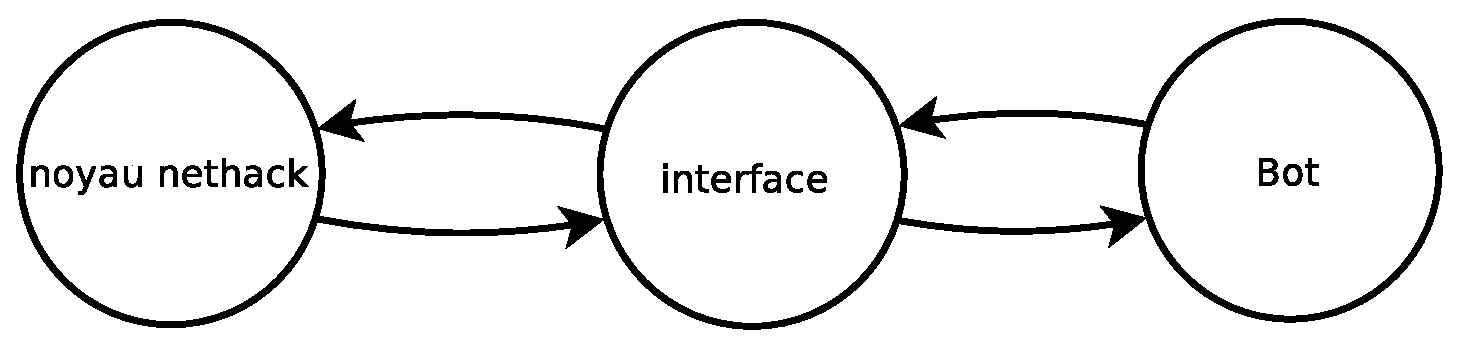
\includegraphics[width=180mm]{diagrammes/proto_archi.eps}
\end{center}

\section{Besoins fonctionnels}

\subsection{Communication avec NetHack}

Le projet doit fournir une interface permettant à des bots de jouer à NetHack. Elle consiste en un module ajouté au jeu assurant la liaison entre le jeu et les différentes parties du projet (bots, base de données, \ldots{}).

Cette interface doit arbitrer les échanges entre les bots et le noyau. Par exemple, elle doit permettre de prouver que les bots ne puissent pas tricher et gérer gracieusement les erreurs provenant des différents programmes intervenants dans la simulation d'une partie.

\subsection{Création de `modes' de jeu}

Le projet devra établir au moins un mode de jeu correspondant à une modification du noyau de NetHack, une liste d'ordres permis aux bots, un ensemble de paramètres introduits à l'exécution et d'informations collectées sur une partie. L'ensemble formant un environnent pour la résolution d'un problème isolé du jeu.

Il sera nécessaire de pouvoir extraire ces modifications afin de permettre leur réapplication sur une verion originale du jeu.

Ce système devra permettre d'exécuter des bots sur le(s) mode(s) établis simplement.

\subsection{Collecte de statistiques}

Le projet devra alimenter une base de données à partir de parties jouées par des bots et des statistiques recueillies. Elles seront utilisées dans un système d'analyse de statistiques.

\subsection{Analyse et présentation des statistiques}

Un outil d'analyse de statistiques devra être livré. Il permettra de comparer entre autres : les performances des bots en termes de taux de réussite et de rapidité de différents algorithmes. Plus généralement, une mesure de pertinence telle que l'écart-type devra être affichée ou intégrée.

Il est souhaitable qu'il intègre un outil générant des graphiques pour une interprétation plus aisée.

\subsection{Outil de replay}

Pour le débogue des bots, il est souhaitable de disposer d'un outil permettant de rejouer une partie ; soit passivement pour identifier une erreur dans l'algorithme d'un bot ; soit activement pour permettre de tester une correction dans l'algorithme d'un bot dans une situation où il avait échoué.

\section{Démarches et études}

Le projet devra se baser sur l'étude de problèmes spécifiques liés au jeu Nethack. L'objectif attendu par le client n'est pas de fournir des bots étant capable de jouer à Nethack, mais au contraire de mettre en place un cadre d'étude de sous-problèmes pouvant être révélés par l'étude du jeu.

Chaque sous-problème sera lié à un ``mode'' de jeu, c'est-à-dire un environnement - défini de façon formelle - dans lequel pourront évoluer des bots spécifiques. Cet environnement est défini par : 
\begin{itemize}
	\item un jeu d'actions autorisées pour les bots (ce jeu d'action est un sous-ensemble du jeu d'action de base) 
	\item la suppression de certaines contraintes telles que la faim, les pièges, etc. 
	\item un sous-ensemble de statistiques prélevée 
	\item un ensemble de paramètre servant à l'évaluation 
	\item des conditions de fin de jeu.
\end{itemize}

Les sous-problèmes suivant pourront faire l'objet d'une étude formelle : 
\begin{itemize}
	\item Exploration d'un niveau.
	\item Recherche de portes secrètes.
	\item Combat.
	\item \ldots
\end{itemize}

Chaque problème fera l'objet d'une approche algorithmique et probabiliste.


\subsection{Recherche de portes secrètes}

Dans le jeu original, une action permet d'effectuer des recherches dans l'environnement du personnage. Cette recherche peut entrainer la découverte de portes secrètes ou de passages secrets. Plusieurs études liées à cette particularité du jeu peuvent être effectuées : 
\begin{itemize}
	\item Avec limite de temps : 
	\begin{itemize}
		\item Comment trouver le plus de portes cachées, le plus vite possible ? 
		\item Comment trouver le plus de portes cachées, dans la limite de temps donnée ? 
		\item etc. 
	\end{itemize}
	\item Sans limite de temps : 
	\begin{itemize}
		\item Comment mettre le moins de temps possible pour trouver toutes les portes ? 
		\item etc.
	\end{itemize}
\end{itemize}

Le mode de jeu correspondant à la recherche des portes secrètes est défini selon les contraintes suivantes : 
\begin{itemize}
	\item Les actions autorisées par le personnage sont limitées aux déplacements, à l'action de recherche, à l'ouverture de portes, au changement de niveau. 
	\item Les contraintes suivantes sont supprimées : 
	\begin{itemize}
		\item la faim, 
		\item les pièges, 
		\item les monstres, 
		\item les objets. 
	\end{itemize}
	\item Les statistiques suivantes sont prélevées : 
	\begin{itemize}
		\item nombre total de portes secrètes, 
		\item nombre de portes secrètes trouvées, 
		\item nombre de tours total, 
	\end{itemize}
	\item La proportion des portes secrètes trouvées et le temps mis pour trouver ces portes seront évalués. 
	\item La fin du jeu aura lieu après une limite de temps donnée ou une fois que toutes les portes secrètes auront été trouvées.
\end{itemize}

\subsection{Exploration d'un niveau}

Ce problème correspond au problèmes de recherche de la sortie d'un labyrinthe.

Différents points peuvent être étudiés : 
\begin{itemize}
	\item Comment sortir le plus rapidement d'un niveau ? 
	\item Comment sortir du niveau en ayant exploré le plus de cases possibles ? 
	\item etc.
\end{itemize}

\section{Besoins non fonctionnels}

Nous avons identifié les spécifications suivantes en terme de contraintes logicielles non fonctionnelles.

\subsection{Choix des sous-problèmes étudiés}

\begin{itemize}
	\item Les bots sont spécialisés dans la résolution d'un problème précis.  L'objectif n'est pas de créer un programme sachant jouer à NetHack dans sa version originale.
	\item Les sous-problèmes étudiés doivent être suffisamment vastes pour envisager plusieurs approches possibles.
\end{itemize}

\subsection{Modifications noyau}

\begin{itemize}
	\item Le code source principal doit être réalisé en langage C, en réutilisant au maximum les fonctionnalités déjà existantes dans NetHack. Ceci ne concerne pas les bots externes ni de potentiels scripts annexes comme un outil d'installation automatique.
	\item Les modifications devront être minimales et justifiées. Des modifications locales d'un nombre de lignes limités sont attendues sous la forme d'un fichier diff.
	\item Les modifications doivent répondre à un besoin d'exécution et ne doivent pas permettre aux bots de tricher.
	\item L'ensemble logiciel doit pouvoir être installé facilement ; si des dépendances extérieures ont été nécessaires, elles doivent être listées et leur installation documentée.
\end{itemize}

\subsection{Interface et création de bots}

\begin{itemize}
\item
  L'interface doit permettre d'introduire de nouveaux bots aisément. Pour cela, le protocole de communication entre le bot et l'interface doit être spécifié. Des ``starter packs'' dans différents langages devront être fournis pour illustrer la démarche de création d'un bot.
\item
  Elle doit permettre de simuler de façon autonome un grand nombre de parties.
\item
  La stratégie employée par les bots doit être explicite. Leur fonctionnement doit soit pouvoir être déduit de leur code, soit documenté par ailleurs.
\end{itemize}

\subsection{Interprétation des statistiques et validation des stratégies}

\begin{itemize}
\item Le déroulement de parties doit fournir des statistiques, dans un format lisible et standard.
\item La production statistique doit pouvoir permettre de valider ou d'infirmer la pertinence de choix stratégiques des bots.
\item La différence de performance entre les bots doit pouvoir être expliquée à l'aide de raisonnements ou d'exemples.
\end{itemize}

\section{Sous-ensemble et priorités d'implémentation}

\begin{itemize}
\item Étudier le code source de NetHack et identifier les mécanismes de créations d'objets, de monstres, etc., afin d'évaluer la difficulté de création des modes.
\item Fournir un moyen de communication entre les bots, le jeu et un système de collecte de données sur les parties jouées.
\item Fournir une première version (éventuellement instable) présentant l'ensemble des fonctionnalités.
\item Produire des statistiques sur les données collectées.
\item Mettre en place au moins deux starter packages dont un en python
\item Développer la fiabilité du logiciel et fournir des versions améliorées des bots.
\item Être capable d'avoir un certain contrôle sur la génération de niveaux adaptés aux problèmes à résoudre.
\item Le développement d'autres modes et d'autres bots se fera pendant le temps restant.
\end{itemize}

\textbf{Diagramme de Gantt à ajouter}

\section{Information de maintenance}

\begin{itemize}
\item De nouveaux modes pourront être ajoutés plus tard dans la vie du logiciel, il convient donc de faire attention à rester libre à l'ajout de modes et de faciliter la création de ceux-ci.
\item De nouveaux bots dans d'autres langages sont susceptibles d'être développés, écrire un starter package doit donc rester simple.
\end{itemize}

\section{Glossaire}

\begin{itemize}
	\item Starter package : Bot volontairement simpliste pouvant servir de base à la création d'un bot sans avoir à réimplémenter les entrées/sorties avec l'interface.
	\item Mode : Configuration spécifique du jeu adaptée à un problème précis. Comprend :
  	\begin{itemize}
		\item Un ensemble de modifications du noyau
		\item Un jeu d'actions possibles avec certaines règles
		\item Un ensemble de paramètre servant à l'évaluation
		\item Des conditions de fin de jeu
  	\end{itemize}
	\item Rogue-like : jeu inspiré du jeu vidéo ``Rogue''. Le joueur incarne un aventurier explorant des souterrains dans lesquels il affronte des monstres tout en se frayant un chemin vers les niveaux inférieurs.
	\item Bot : programme informatique automatisant des actions dans un jeu ou simulant un joueur humain
\end{itemize}

\end{document}

%vim:tw=0
